\begin{frame}{New Experiment: Is It Just the Low Temperature?}
\begin{columns}[c]
\begin{column}{0.58\textwidth}
\uncover<2->{\begin{figure}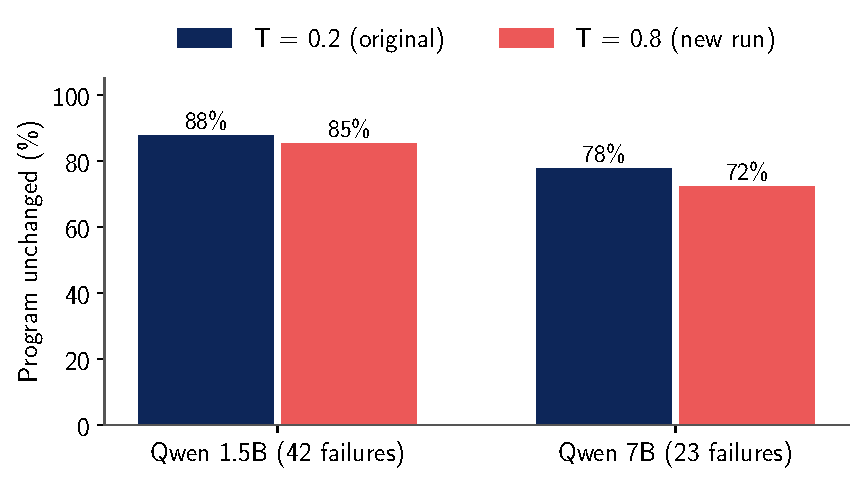
\includegraphics[width=0.92\linewidth]{figs/temperature.pdf}
\caption{Full-history repair rerun at $T=0.8$ from the same failed programs (seed 11)}\end{figure}}
\end{column}
\begin{column}{0.4\textwidth}
\footnotesize
\begin{itemize}\setlength{\itemsep}{0.2em}
\item Objection: at $T=0.2$ the model is too deterministic to change its code
\item Test: rerun every repair at $T=0.8$ from the same failed answers
\item<2-> Still \hl{85\%} (1.5B) and \hl{72\%} (7B) unchanged
\item<3-> Correct after repair (hidden tests): 2 $\to$ 2 (1.5B), 1 $\to$ 2 (7B)
\end{itemize}
\uncover<4->{\begin{keybox}{Insight}Not randomness: the model is \textbf{confident in its wrong answer}.\end{keybox}}
\end{column}
\end{columns}
\end{frame}

\begin{frame}{Live Demo: Repair vs.\ Fresh Retry}
\small Same problem (HumanEval/134), Qwen 1.5B, laptop GPU:\\ \texttt{python live\_demo.py -{}-task HumanEval/134}
\vspace{0.6em}
\begin{columns}[T]
\begin{column}{0.48\textwidth}
\begin{defbox}{Repair with feedback}
\begin{tabular}{@{}lll@{}}
Attempt & Visible tests & Energy\\
\midrule
1 & 9/10 \textcolor{accent}{fail} & 84.5\,J\\
2 & 9/10 \textcolor{accent}{fail} & 96.4\,J\\
3 & 9/10 \textcolor{accent}{fail} & 100.3\,J\\
4 & 9/10 \textcolor{accent}{fail} & 90.9\,J\\
\midrule
\multicolumn{2}{@{}l}{\textbf{Same program 4 times}} & \textbf{372\,J}
\end{tabular}
\end{defbox}
\end{column}
\begin{column}{0.48\textwidth}
\uncover<2->{%
\begin{exbox}{Fresh retry}
\begin{tabular}{@{}lll@{}}
Attempt & Visible tests & Energy\\
\midrule
1 & 9/10 \textcolor{accent}{fail} & 77.0\,J\\
2 & 10/10 \textcolor{teal}{pass} & 96.4\,J\\
\midrule
\multicolumn{2}{@{}l}{\textbf{Solved in 2 attempts}} & \textbf{173\,J}
\end{tabular}
\end{exbox}}
\end{column}
\end{columns}
\vspace{0.4em}
\uncover<3->{\src{Rehearsal run, 21 November 2026. Energy varies run to run; the pattern is the point.}}
\end{frame}
